% Journal class not chosen yet: two-column article + natbib for now.
\documentclass[10pt,twocolumn]{article}

\usepackage[utf8]{inputenc}
\usepackage[T1]{fontenc}
\usepackage{amsmath,amssymb}
\usepackage{graphicx}
\usepackage{booktabs}
\usepackage{xspace}
\usepackage[authoryear,round]{natbib}
\usepackage[colorlinks=true,citecolor=blue,linkcolor=blue,urlcolor=blue]{hyperref}
\usepackage[margin=2cm,columnsep=0.7cm]{geometry}

\graphicspath{{figures/}}

% Symbols used throughout (as in the ULXspectra README)
\newcommand{\mdot}{\dot m}
\newcommand{\Mdot}{\dot M}
\newcommand{\Rsph}{R_{\rm sph}}
\newcommand{\Rtrap}{R_{\rm trap}}
\newcommand{\rin}{r_{\rm in}}
\newcommand{\rout}{r_{\rm out}}
\newcommand{\rg}{r_{\rm g}}
\newcommand{\rmag}{r_{\rm m}}
\newcommand{\RNS}{R_{\rm NS}}
\newcommand{\Rref}{R_{\rm ref}}
\newcommand{\Teff}{T_{\rm eff}}
\newcommand{\Tw}{T_{\rm w}}
\newcommand{\LEdd}{L_{\rm Edd}}
\newcommand{\MEdd}{\dot M_{\rm Edd}}
\newcommand{\etaEdd}{\eta_{\rm Edd}}
\newcommand{\kT}{\kappa_{\rm T}}
\newcommand{\Fvis}{F_{\rm vis}}
\newcommand{\Qvis}{Q_{\rm vis}}
\newcommand{\xsp}{x_{\rm sph}}
\newcommand{\xeff}{x_{\rm eff}}
\newcommand{\taup}{\tau_\perp}
\newcommand{\hd}{h_{\rm disc}}
\newcommand{\omf}{\omega_{\rm frac}}
\newcommand{\vK}{v_{\rm K}}
\newcommand{\code}[1]{\texttt{#1}}

% Source names (the code calls them HolmIX, NGC1313B, NGC5408)
\newcommand{\srcHoIX}{Holmberg~IX X-1\xspace}
\newcommand{\srcNGCthirteen}{NGC1313B\xspace}
% AUTHOR: full name of NGC1313B (decide later)
\newcommand{\srcNGCfiftyfour}{NGC~5408 X-1\xspace}

\title{Spectra of ultraluminous X-ray sources from a supercritical disc with an optically thick wind}
% Working title
\author{G.~Lipunova$^{1,2}$ \and C.~Pinto$^{3}$ \and P.~Abolmasov$^{4}$ \and V.~Ahlberg$^{4}$ \\[1ex]
\parbox{0.9\textwidth}{\centering\small
$^1$Dr.~Karl Remeis-Observatory and Erlangen Centre for Astroparticle Physics, Friedrich-Alexander-Universit\"at Erlangen-N\"urnberg, Sternwartstr.~7, 96049 Bamberg \\
$^2$Max-Planck-Institut f\"ur Radioastronomie, Auf dem H\"ugel 69, 53121 Bonn \\
$^3$AFFILIATION MISSING \\
$^4$AFFILIATION MISSING}}
% Authors and affiliations from the old manuscript (SEA_spectrum.zip, main.tex); there
% institutes 3 and 4 are referenced but not listed. VERIFY: affiliations 3 and 4, author order.
\date{Draft, \today}

\renewcommand{\abstractname}{Summary}

\begin{document}

\twocolumn[
\begin{@twocolumnfalse}
\maketitle
\begin{abstract}
% Sources: README "Model Physics" (intro); results pending
% Draft of the model part only; the results part waits for the full-range fits.

We present a model of the broadband spectrum, from the optical to the X-rays, of a supercritical accretion disc with an optically thick wind around a black hole, or around a neutron star with a magnetosphere.
Inside the spherization radius the disc loses mass to a wind launched along straight streamlines, and the accretion rate falls towards the centre.
Inside the trapping radius advection makes the effective temperature fall as $R^{-1/2}$.
The wind photosphere is found from the streamline density, and its temperature from the advection of photons by the wind together with the energy that the disc releases but does not show directly.
For a neutron star, the matter inside the magnetospheric radius radiates from a sphere or from the surface of the last closed dipole field line.
The observed spectrum is the sum of blackbodies over the visible surface at the inclination of the observer, with occultation by the wind and the disc.
% OUTLINE: Fits to the SEDs of the selected ULXs: method (MCMC) and main results.

\end{abstract}
\vspace{1em}
\end{@twocolumnfalse}
]

% Sources: author

\section{Introduction}
\label{sec:intro}

% OUTLINE: ULXs and super-Eddington accretion; BH and NS (pulsating ULX) accretors.
% OUTLINE: Supercritical discs with outflows: SS73, L99, P07; review by Middleton et
%          al. (2026).
% OUTLINE: What this work adds: a model computing the broadband spectrum (optical to
%          X-rays) of disc + wind + central emitter, with the wind photosphere from a
%          streamline density; fits to observed SEDs.
% OUTLINE: Structure of the paper.

% Sources: README "Model Physics" (intro), "Units and radii", "Wind scenarios and the accretion-rate profile"
% Code: ULXspectra, branch fix-results-integrity, commit 5f00569

\section{Model overview}
\label{sec:model}

\subsection{Geometry and order of the calculation}
\label{sec:model:geometry}

The accretor is a black hole (BH) or a neutron star (NS) with a magnetosphere.
Matter arrives at the outer disc radius at a constant rate $\Mdot_0$.
Inside the spherization radius $\Rsph$ part of it leaves the disc in a wind, so that the accretion rate $\Mdot(R)$ falls towards the inner disc radius $\rin$.
The wind fills the cone between the funnel, the innermost streamline at angle $\theta_{\rm c}$ to the axis, and the disc surface.
For a NS, the matter inside $\rin = \rmag$ radiates from the magnetosphere, which we call the central emitter.
% OUTLINE: sketch figure of the geometry (disc, wind cone, funnel, photosphere,
%          outer wall, central emitter, observer at inclination i). AUTHOR: make or
%          provide; it must come from a script in the code repository.

The calculation goes through these steps in order:
\begin{enumerate}
\item radii and units (this section);
\item $\Mdot(R)$, $\Rsph$ and the trapping radius $\Rtrap$ (Sects.~\ref{sec:model:mdot} and~\ref{sec:radii});
\item viscous torque and disc effective temperature (Sect.~\ref{sec:disc});
\item luminosity budget of the disc and the central emitter (Sect.~\ref{sec:disc:budget});
\item the NS magnetosphere (Sect.~\ref{sec:central});
\item wind streamlines, density and photosphere (Sect.~\ref{sec:wind});
\item wind temperature and its energy budget (Sect.~\ref{sec:wtemp});
\item visibility and spectrum (Sect.~\ref{sec:spectrum}).
\end{enumerate}
% Source: README "Model Physics", steps 1-8.

\subsection{Units and radii}
\label{sec:model:units}

The Eddington luminosity is
\begin{equation}
\LEdd = \frac{4\pi G M c}{\kT}, \qquad \kT = 0.34~{\rm cm^2\,g^{-1}},
\label{eq:LEdd}
\end{equation}
% code: README "Units and radii"; KAPPA_T_CGS in csrcs
and the Eddington accretion rate is
\begin{equation}
\MEdd = \frac{\LEdd}{\etaEdd\, c^2}, \qquad \mdot = \frac{\Mdot}{\MEdd}.
\label{eq:MEdd}
\end{equation}
% code: README "Units and radii"; eta_edd_of() (csrcs/disc_struct.c)
We take $\etaEdd = 1/12$, that is $\MEdd = 12\,\LEdd/c^2$, as in \citet{Poutanen2007} and \citet{Lipunova1999}; \citet{Middleton2026} use $\etaEdd = 1/10$.
The outer accretion rate is $\mdot_0$.
% AUTHOR: one sentence on why 1/12 (e.g. efficiency of a Newtonian disc with
%         r_in = 6 r_g)? The sources only say "as in P07 and L99".

Radii are measured in $\rg = GM/c^2$, and in the code in units of the inner disc radius, $x = R/\rin$.
For a BH, $\rin = r_{\rm in,f}\,\rg$, where $r_{\rm in,f}$ (\code{r\_in\_factor}) is a free parameter.
For a NS, the inner disc radius is the magnetospheric radius,
\begin{equation}
\rin = \rmag = x_{\rm m}\, r_{\rm in,f}\, \rg ,
\label{eq:rm}
\end{equation}
% code: apply_physical_radii() (csrcs/disc_struct.c); README "Units and radii"
where $x_{\rm m}$ is \code{wind\_inner\_launch\_x}; only the product of the two factors matters.
The prior rejects $\rmag \le \RNS = 10$~km.
In both cases the wind is launched from $\rin$ outwards.
% AUTHOR: the code names (wind_inner_launch_x, r_in_factor) are historical; is the
%         paper notation r_in,f and x_m fine, or would you parametrise the NS by r_m
%         directly?

The flow rules of \citet{Poutanen2007} and \citet{Shakura1973} (Sect.~\ref{sec:model:mdot}) are fixed in units of $\rg$ through the reference radius $\Rref = 6\,\rg$, the innermost stable circular orbit of a non-rotating BH and the inner radius $3R_{\rm S}$ of \citet{Poutanen2007}.
The actual inner disc radius only truncates them.
% code: R_IN_REF_FACTOR (csrcs); README "Units and radii"

The outer disc radius $\rout$ is free.
Only the disc inside $\rout$ emits and counts in the disc luminosity.
If $\rout$ lies inside the outer wall of the wind (Sect.~\ref{sec:wind:photosphere}), the disc there is hidden but still sets the wind temperature (Sect.~\ref{sec:wtemp}); beyond the wall the outer disc is seen directly.
The radial grid extends to $\max(10^4\mdot_0\,\rin, \rout)$; the rings beyond $\rout$ do not emit but can occult.
% code: README "Units and radii"; radial_grid_edges() (csrcs/wind_surface.c)

\subsection{Accretion rate in the disc}
\label{sec:model:mdot}

Outside $\Rsph$ the accretion rate is constant, $\mdot = \mdot_0$.
For $\mdot_0 \le 1$ there is no wind and $\Rsph = \rin$ (Sect.~\ref{sec:radii}).
Inside $\Rsph$ the main model of this paper prescribes the fraction $f_{\rm in} = \mdot(\rin)/\mdot_0$ (\code{user\_mdot\_in\_fraction}) that reaches the inner disc radius, and takes $\Mdot$ linear in $R$ between $\rin$ and $\Rsph$:
\begin{equation}
\mdot(x) = \mdot_0 \left[ f_{\rm in} + (1 - f_{\rm in})\,\frac{x - 1}{\xsp - 1} \right]
\label{eq:mdot_setin}
\end{equation}
% code: mdot_acc_profile_scalar(), branch "set_mdot_in" (csrcs/disc_struct.c); README "Wind scenarios"
for $1 \le x < \xsp$, with $\xsp = \Rsph/\rin$.
$f_{\rm in}$ is free in the fits.
% AUTHOR: motivation for the linear profile and for leaving f_in free (vs P07 eq. 23,
%         which fixes it through eps_w)?

We compare this model with three flow rules from the literature, selected in the code by \code{wind\_scenario} (Table~\ref{tab:presets}).
In the profile of \citet[][hereafter P07]{Poutanen2007}, $\Mdot$ is linear in $u = R/\Rref$,
\begin{equation}
\mdot = \mdot_{\rm in} + (\mdot_0 - \mdot_{\rm in})\,\frac{u - 1}{u_{\rm sph} - 1}, \qquad u < u_{\rm sph},
\label{eq:mdot_P07}
\end{equation}
% code: mdot_acc_profile_scalar(), branch "P07" (csrcs/disc_struct.c); README "Wind scenarios"
with the inner rate set by the wind energy fraction $\epsilon_{\rm w}$ (P07, eq.~23),
\begin{equation}
\frac{\mdot_{\rm in}}{\mdot_0} = \frac{1 - a}{1 - a/\sqrt{2\mdot_0/5}},
\label{eq:mdot_in_P07}
\end{equation}
% code: mdot_in_over_mdot0(), a_ew() (csrcs/disc_struct.c); README "Wind scenarios"
where $a = \epsilon_{\rm w}(0.83 - 0.25\,\epsilon_{\rm w})$.
The profile is evaluated at $\max(R, \rin)$ and is not allowed to become negative.
The L99 preset is the P07 profile with $\epsilon_{\rm w} = 1$ \citep{Lipunova1999}.
In the profile of \citet[][SS73]{Shakura1973},
\begin{equation}
\mdot = \mdot_0\,\frac{R}{\Rsph}, \qquad R < \Rsph .
\label{eq:mdot_SS73}
\end{equation}
% code: mdot_acc_profile_scalar(), branch "SS73"; mdot_in_over_mdot0() gives x_launch/x_sp
% AUTHOR: check that the P07 eq. 23 and the attribution of eq. (mdot_SS73) to SS73
%         are as you want them cited.

\begin{table*}
\centering
\caption{Flow rules (\code{wind\_scenario}). The presets of the literature fix the $\Mdot(R)$ profile, the $\Rsph$ rule and $\etaEdd$; $\Rtrap$ can be set in any of them.}
\label{tab:presets}
\small
\begin{tabular}{@{}lllll@{}}
\toprule
Preset & $\Mdot(R)$ & $\Rsph$ & $\etaEdd$ & $\Rtrap$ \\
\midrule
main (\code{set\_mdot\_in}) & Eq.~\eqref{eq:mdot_setin} & free & 1/12 & M26 \\
P07 & Eq.~\eqref{eq:mdot_P07} & P07fit & 1/12 & M26 \\
L99 & Eq.~\eqref{eq:mdot_P07}, $\epsilon_{\rm w}=1$ & P07fit & 1/12 & M26 \\
SS73 & Eq.~\eqref{eq:mdot_SS73} & SS73, SS73\_eq71 & 1/12 & $\Rsph$ \\
\bottomrule
\end{tabular}
% code: psrcs/flow_rules.py PAPER_PRESETS, resolve_flow_rules(); README table "Wind scenarios"
% Rules named in the R_sph and R_trap columns: Sect. radii.
\end{table*}

\subsection{Mass loss}
\label{sec:model:massloss}

The wind carries away
\begin{equation}
\Mdot_{\rm w}(R) = \Mdot(R) - \Mdot(\rin),
\label{eq:Mdotw}
\end{equation}
% code: mdot_wind_cumulative_scalar() (csrcs/wind_struct.c); README "Wind scenarios"
the mass launched between $\rin$ and $R$.
The rate of mass loss per unit area of each side of the disc at the launch radius $R_0$ is
\begin{equation}
\dot\Sigma_{\rm w}(R_0) = \frac{1}{4\pi R_0}\,\frac{{\rm d}\Mdot_{\rm w}}{{\rm d}R_0} .
\label{eq:Sigmadotw}
\end{equation}
% code: make_dotSigma_table() (csrcs/wind_struct.c); README "Wind scenarios"
For the main model, $\dot\Sigma_{\rm w} \propto 1/R_0$ between $\rin$ and $\Rsph$.

\subsection{Parameters}
\label{sec:model:params}

Table~\ref{tab:params} lists the parameters of the model.
% OUTLINE: say which parameters are free in which fit (BH1/BH3/BH4/NS1 presets of
%          ULX.conf), once the set of fits for the paper is fixed.

\begin{table*}
\centering
\caption{Physical parameters. Default values and prior ranges are those of \code{ULX.conf}; free parameters have flat priors in the range given.}
\label{tab:params}
\small
\begin{tabular}{@{}lllll@{}}
\toprule
Symbol & Code name & Meaning & Default & Prior \\
\midrule
$\log M/M_\odot$ & \code{log\_m\_bh} & mass of the accretor & 1.0 & (0, 4) \\
$\log \mdot_0$ & \code{log\_mdot0} & outer accretion rate, units of $\MEdd$ & 2.0 & (0, 5) \\
$f_{\rm in}$ & \code{user\_mdot\_in\_fraction} & $\mdot(\rin)/\mdot_0$, main model & 0.5 & (0, 1) \\
$r_{\rm in,f}$ & \code{r\_in\_factor} & $\rin/\rg$ (BH), $\rmag/(x_{\rm m}\rg)$ (NS) & 6 & (1, 20) \\
$\log x_{\rm m}$ & \code{log\_wind\_inner\_launch\_x} & NS: $\rmag$ in units of $r_{\rm in,f}\rg$; BH: 0 & 0 & (0, 4) \\
$\log \rout/\rg$ & \code{log\_r\_out\_factor} & outer disc radius & 5.0 & (2, 10) \\
$i$ & \code{incl\_deg} & inclination, degrees & 20 & (0, 88) \\
$\epsilon_{\rm w}$ & \code{eps\_w} & fraction of the energy spent on launching the wind & 0.5 & ($10^{-4}$, 0.999) \\
$\beta_{\rm w}$ & \code{beta\_w} & wind speed at infinity, units of $\vK(R_0)$ & 1.0 & (0.05, 3) \\
$\omf$ & \code{omega\_frac} & $\cos\theta_{\rm c} - \cos\theta_{\rm d}$, solid-angle fraction of the wind & 0.7 & (0.1, 0.85) \\
$\hd$ & \code{h\_disc} & disc surface $z/R$ & 0 & (0, 0.3) \\
$\log\eta_{\rm magn}$ & \code{log\_magn\_eta} & NS: efficiency of the central emitter & 0 & ($-5$, 0) \\
$\beta_{\rm t}$ & \code{beta\_torque\_in} & NS: torque at $\rmag$ & 1 & fixed \\
$z/r$ & \code{z\_over\_r\_trap} & disc thickness in $\Rtrap$ & 0.5 & fixed \\
\bottomrule
\end{tabular}
% code: ULX.conf [DEFAULT] at commit 5f00569; README "Physical Parameters".
% Discrete switches (not in the table): wind_scenario, rsp_rule, rtrap_rule,
% disc_luminosity_mode (1+log for BH, NS), dip, wind_velocity_law (ballistic).
\end{table*}

% Sources: README "Spherization radius", "Trapping radius"
% Code: ULXspectra, branch fix-results-integrity, commit 5f00569

\section{Spherization and trapping radii}
\label{sec:radii}

\subsection{Spherization radius}
\label{sec:radii:sph}

For $\mdot_0 \le 1$ there is no wind and $\Rsph = \rin$.
Otherwise $\Rsph$ follows from one of the rules in Table~\ref{tab:rsph}, and it is never below $\rin$.
% code: rsp_over_rin() (csrcs/disc_struct.c); README "Spherization radius"

\begin{table}
\centering
\caption{Rules for the spherization radius (\code{rsp\_rule}).}
\label{tab:rsph}
\small
\begin{tabular}{@{}ll@{}}
\toprule
Rule & $\Rsph$ \\
\midrule
P07fit & Eq.~\eqref{eq:rsph_P07} \\
SS73 & $\Rref\,\mdot_0$ \\
SS73\_eq71 & $(9/4)\,\Rref\,\mdot_0$ \\
M26 & $1.5\,(\mdot_0/\etaEdd)\,\rg$ \\
Ledd & Eq.~\eqref{eq:rsph_Ledd} \\
mdot0 & $\mdot_0\,\rin$ \\
\bottomrule
\end{tabular}
% code: rsp_over_rin() (csrcs/disc_struct.c); README table "Spherization radius"
\end{table}

P07 give a fit to their numerical solutions (P07, eq.~21),
\begin{equation}
\begin{split}
\frac{\Rsph}{\Rref} = \mdot_0 \bigl[ & 1.34 - 0.4\,\epsilon_{\rm w} + 0.1\,\epsilon_{\rm w}^2 \\
& - (1.1 - 0.7\,\epsilon_{\rm w})\,\mdot_0^{-2/3} \bigr].
\end{split}
\label{eq:rsph_P07}
\end{equation}
% code: rsp_over_rin(), rule "P07fit" (csrcs/disc_struct.c); README "Spherization radius"
For the SS73 profile, the rule \code{SS73} places $\Rsph$ where $\mdot(\Rref) = 1$ in Eq.~\eqref{eq:mdot_SS73}, and \code{SS73\_eq71} takes eq.~(7.1) of \citet{Shakura1973} literally.
The rule \code{M26} is $\Rsph = (3/8\pi)\,\kT\Mdot_0/c$ \citep{Middleton2026}.
The rule \code{mdot0} sets $\Rsph = \mdot_0\,\rin$, so that it scales with the actual inner radius rather than with $\Rref$.
% code: rsp_over_rin(), rules "SS73", "SS73_eq71", "M26", "mdot0"

The rule \code{Ledd} follows \citet{Lipunova1999}: $\Rsph$ is the radius outside which the disc releases $\LEdd$.
With the viscous torque of Sect.~\ref{sec:disc:torque} and $\Mdot = \Mdot_0$ outside $\Rsph$, the luminosity of both sides of the disc beyond $\Rsph$ is $\Fvis(\Rsph)\,\Omega_{\rm K}(\Rsph) + G M \Mdot_0/(2\Rsph)$, so the condition reads
\begin{equation}
\Fvis(\Rsph)\,\Omega_{\rm K}(\Rsph) + \frac{G M \Mdot_0}{2\Rsph} = \LEdd ,
\label{eq:rsph_Ledd}
\end{equation}
% code: rsp_self_consistent_x(), rsp_self_consistent_func() (csrcs/disc_struct.c),
%       which solve the same equation divided by Mdot_in G M / r_in, in t = sqrt(x_sph).
% source: old manuscript (SEA_spectrum.zip, main.tex, "Derivation of R_sp"; Rsp_reasoning.txt sects. 3-5),
%       L_out = (GM)^2 [F_sp/h_sp^3 + Mdot_0/(2 h_sp^2)], the same expression.
where $\Omega_{\rm K} = \sqrt{GM/R^3}$ and $\Fvis(\Rsph)$ is given by Eq.~\eqref{eq:Fvis_lin} with $F_{\rm in} = 0$.
$\Fvis(\Rsph)$ depends on $\Rsph$ through the profile~\eqref{eq:mdot_setin}.
With $t = (\Rsph/\rin)^{1/2}$ and $q = 1/f_{\rm in}$, Eq.~\eqref{eq:rsph_Ledd} becomes a quartic equation,
\begin{equation}
\begin{split}
6\lambda t^4 + 6\lambda t^3 - (4 + 5q)\,t^2 - (5q - 2)\,t + 4q + 2 &= 0, \\
\lambda = \frac{\LEdd\,\rin}{GM\Mdot(\rin)} = \frac{\etaEdd\,\rin}{f_{\rm in}\mdot_0\,\rg} & ,
\end{split}
\label{eq:rsph_quartic}
\end{equation}
% source: Rsp_reasoning.txt sect. 6 (in SEA_spectrum.zip), with f = F_in/(Mdot_in h_in) = 0 and x_w = 1;
% checked numerically (Claude): equals -6 (t+1) t^3 [F_sph/(Mdot_in h_in t^3) + q/(2 t^2) - lambda]
% code: rsp_self_consistent_x() solves the unexpanded form by bisection (csrcs/disc_struct.c)
whose root $t \ge 1$ we find numerically.
It depends on the actual inner radius and is implemented only for the main profile~\eqref{eq:mdot_setin}.
If the disc is already below $\LEdd$ beyond $\rin$, $\Rsph = \rin$.
% code: rsp_self_consistent_x(): returns x_launch if f(1) < 0; NaN for other profiles in rsp_over_rin()
% AUTHOR: the code uses F_in = 0 in eq. (rsph_Ledd) also for a NS
%         (RSP_SELF_CONSISTENT_F_IN = 0), while the disc torque has F_in = beta Mdot_in h_in.
%         Intended? Then the text should say so.

% AUTHOR: which R_sph rule(s) belong to the main model? The set_mdot_in fits use
%         three: mdot0 (BH1, BH3, BH4, NS3: use_simple_rsp = 1), Ledd (BH1a, BH3a,
%         BH4a, NS1a, NS6: use_simple_rsp = 2), and P07fit (NS1: default 0).
%         ULX.conf still says "TODO decide use_simple_rsp". The text above presents
%         all rules on equal footing until you decide.

\subsection{Trapping radius}
\label{sec:radii:trap}

Inside the trapping radius, photons are advected with the flow and the disc effective temperature falls as $R^{-1/2}$ (Sect.~\ref{sec:disc:teff}).
Following \citet{Middleton2026} we take
\begin{equation}
\Rtrap = 2\,\frac{z}{r}\,\frac{\mdot_0}{\etaEdd}\,\rg ,
\label{eq:rtrap}
\end{equation}
% code: rtrap_over_rin(), rule "M26" (csrcs/disc_struct.c); README "Trapping radius"
with the disc thickness $z/r = 0.5$, which gives $\Rtrap = 12\,\mdot_0\,\rg$ for $\etaEdd = 1/12$.
For the SS73 preset we set $\Rtrap = \Rsph$ instead.
SS73 have no advection, but inside $\Rsph$ their outflow also gives $\Teff \propto R^{-1/2}$.
% code: rtrap_over_rin(), rule "rsp"; psrcs/flow_rules.py (SS73 default rtrap_rule = rsp)
Indeed, with $\Mdot \propto R$ (Eq.~\ref{eq:mdot_SS73}) and $F_{\rm in} = 0$, Eq.~\eqref{eq:Fvis} gives $\Fvis = \Mdot_0\,(Rh - \rin h_{\rm in})/(3\Rsph)$, and far from $\rin$
\begin{equation}
\Qvis \approx \frac{GM\Mdot(R)}{8\pi R^3} \propto R^{-2} .
\label{eq:Qvis_SS73}
\end{equation}
% source: old manuscript (SEA_spectrum.zip, main.tex, Sect. "Effective temperature distribution", eqs. Mdot_SS, F_SS);
%         checked: int Mdot_0 (R/R_sph) dh = Mdot_0 R h/(3 R_sph)
$\Rtrap$ is never below $\rin$; sub-Eddington rates usually give $\Rtrap \le \rin$, that is a standard disc without trapping.
% code: rtrap_over_rin() (fmax with x_launch and 1); README "Trapping radius"
% AUTHOR: z/r = 0.5 is the code default; is it fixed for the paper?

% Sources: README "Viscous torque and disc temperature", "Luminosity budget"
% Code: ULXspectra, branch fix-results-integrity, commit 5f00569

\section{Disc structure and luminosity budget}
\label{sec:disc}

\subsection{Viscous torque}
\label{sec:disc:torque}

Let $h = \sqrt{GMR}$ be the specific angular momentum of the Keplerian disc and $\Fvis > 0$ the viscous torque.
If the matter lost to the wind at $R$ carries away the specific angular momentum $k_{\rm w}h(R)$, the conservation of angular momentum in a stationary disc reads
\begin{equation}
\frac{{\rm d}(\Mdot h)}{{\rm d}R} - \frac{{\rm d}\Fvis}{{\rm d}R} - k_{\rm w}\,h\,\frac{{\rm d}\Mdot}{{\rm d}R} = 0 .
\label{eq:angmom}
\end{equation}
% source: old manuscript (SEA_spectrum.zip, main.tex, Sect. "Effective temperature distribution"),
%         there written for F = -F_vis; code: disc_Fvis_point() (csrcs/disc_struct.c) assumes k_w = 1
We take $k_{\rm w} = 1$, that is, the wind removes the Keplerian angular momentum of the radius where it is launched.
Then the viscous torque obeys
\begin{equation}
\frac{{\rm d}\Fvis}{{\rm d}h} = \Mdot(R), \quad \Fvis(R) = F_{\rm in} + \int_{h(\rin)}^{h(R)} \!\Mdot\,{\rm d}h .
\label{eq:Fvis}
\end{equation}
% code: disc_Fvis_point() (csrcs/disc_struct.c); README "Viscous torque and disc temperature"; PLAN C10
For a BH the torque vanishes at the inner radius, $F_{\rm in} = 0$.
For a NS, the magnetosphere exerts a torque at $\rmag$,
\begin{equation}
F_{\rm in} = \beta_{\rm t}\,\Mdot(\rmag)\,h(\rmag),
\label{eq:Fin_NS}
\end{equation}
% code: disc_Fvis_point() (csrcs/disc_struct.c); README "Viscous torque and disc temperature"
with $\beta_{\rm t} = 1$.
% AUTHOR: physical justification of beta_t = 1 (PLAN C10)?

All the profiles of Sect.~\ref{sec:model:mdot} are linear in $R$ between $\rin$ and $\Rsph$, so the integral is analytic.
With $s = \sqrt{\min(x, \xsp)}$ and $h_{\rm in} = h(\rin)$,
\begin{multline}
\Fvis = F_{\rm in} + \frac{h_{\rm in}(s - 1)}{3(s + 1)}\bigl[\Mdot(\rin)(2s + 1) \\
+ \Mdot(s^2\rin)(s + 2)\bigr]
+ \Mdot_0\,\bigl[h(R) - h(\Rsph)\bigr]\,\Theta(R - \Rsph),
\label{eq:Fvis_lin}
\end{multline}
% code: disc_Fvis_point() (csrcs/disc_struct.c), closed form in its header comment
where $\Theta$ is the Heaviside step function.
$\Fvis$ and the disc temperature are continuous at $\Rsph$.

Since the wind takes away angular momentum, less of it has to be transported by the viscous stress, and it is the stress that heats the disc.
Outside $\Rsph$ the torque is lower than in a disc without outflow and with the same $\Mdot_0$ by $\int (\Mdot_0 - \Mdot)\,{\rm d}h$, taken from $\rin$ to $\Rsph$, so the outer disc is colder.
% source: old manuscript (SEA_spectrum.zip, main.tex), paragraph "Worth noting that the presence of the wind makes the disc colder"
% derived (Claude): the difference follows from eq. (Fvis) with F_in equal in both discs.
% AUTHOR: the old manuscript marks the paragraph before this one "somehow wrong: see the
%         figure" (Fvis_comp.png: SS73 torque vs. an advective disc with outflow). Is the
%         statement above unaffected?
The relative difference fades at $R \gg \Rsph$, where $\Fvis \approx \Mdot_0 h$ in both discs.
% derived (Claude)
% AUTHOR (minor): for P07 with r_in,f < 6 the profile can be clipped at 0 near r_in;
%         the code ignores that non-linear piece (comment in disc_Fvis_point()).
%         Mention or not?

\subsection{Effective temperature}
\label{sec:disc:teff}

The viscous heating per unit area of one side of the disc is
\begin{equation}
\Qvis = \frac{3}{8\pi}\,\frac{\Fvis\,\Omega_{\rm K}}{R^2} .
\label{eq:Qvis}
\end{equation}
% code: disc_Qvis_point() (csrcs/disc_struct.c); README "Viscous torque and disc temperature"
Outside the trapping radius the disc radiates locally, $\sigma\Teff^4 = \Qvis$.
Inside it, advection makes the radiated flux fall as $R^{-2}$, and we join the two continuously at $\Rtrap$:
\begin{equation}
\sigma\Teff^4 =
\begin{cases}
\Qvis(R), & R > \Rtrap, \\
\Qvis(\Rtrap)\,(\Rtrap/R)^2, & \rin \le R \le \Rtrap .
\end{cases}
\label{eq:Teff}
\end{equation}
% code: disc_Qvis_and_Teff() (csrcs/disc_struct.c); README "Viscous torque and disc temperature"
$\Qvis(\Rtrap)$ is evaluated as if the disc continued beyond $\rout$.
% AUTHOR: physical argument for sigma T^4 ~ R^-2 inside R_trap (L_per ln R = const),
%         with a reference?

\subsection{Luminosity budget}
\label{sec:disc:budget}

The disc luminosity is the integral of the profile~\eqref{eq:Teff} over both sides of the disc from $\rin$ to $\rout$:
\begin{multline}
L_{\rm disc} = 4\pi\int_{\rin}^{\rout} \sigma\Teff^4\,R\,{\rm d}R
= L_{\rm vis}(\Rtrap, \rout) \\
+ 4\pi\Rtrap^2\,\Qvis(\Rtrap)\,\ln\frac{\min(\Rtrap, \rout)}{\rin},
\label{eq:Ldisc}
\end{multline}
% code: accretion_luminosity_split(), disc_L_out_above(), disc_advective_L_per_lnr() (csrcs/wind_emission.c, csrcs/disc_struct.c); README "Luminosity budget"
where $L_{\rm vis}(\Rtrap, \rout) = 4\pi\int \Qvis R\,{\rm d}R$ is the viscous release between $\Rtrap$ and $\rout$.
For $\Rtrap \le \rin$ this is the whole viscous release, which also covers sub-Eddington rates.
When $\Rtrap$ is close to the radius outside which the disc releases $\LEdd$, Eq.~\eqref{eq:Ldisc} gives $L_{\rm disc} \approx \LEdd[1 + \ln(\Rtrap/\rin)]$.
% code: README "Luminosity budget", mode 1+log

For a BH, nothing inside $\rin$ radiates.
For a NS, the matter reaching $\rmag$ falls onto the star along the field lines and releases
\begin{equation}
L_{\rm central} = \eta_{\rm magn}\,G M\,\Mdot(\rmag)\left(\frac{1}{\RNS} - \frac{1}{\rmag}\right),
\label{eq:Lcentral}
\end{equation}
% code: accretion_luminosity_split(), mode "NS" (csrcs/wind_emission.c); README "Luminosity budget"
with the efficiency $\eta_{\rm magn} \le 1$, which covers losses such as outflows from the magnetosphere.
The Keplerian kinetic energy of the matter at $\rmag$, about $GM\Mdot/(2\rmag)$, is not counted: for a slow rotator it would also be released inside, while near spin equilibrium it goes partly into the spin of the star.
% code: comment at accretion_luminosity_split() (csrcs/wind_emission.c)
% AUTHOR: check that this is how you want the omission justified.
The total accretion luminosity is $L_{\rm acc} = L_{\rm disc} + L_{\rm central}$.
% code: diagnostic Lbol_accr_teor

% Sources: README "Central emitter (NS magnetosphere)"

\section{Central emitter: the NS magnetosphere}
\label{sec:central}

% OUTLINE: dip = 0 sphere of radius r_m; dip = 1 surface of the last closed dipole
%          field line, z = w^(2/3) sqrt(1 - w^(2/3)). code:
%          dipole_spherical_radius().
% OUTLINE: Temperature along the field line, normalisation to L_central (magn_eta);
%          dark when the budget is zero.
% OUTLINE: Radial grid with x = 1 as a bin edge (C16). code: radial_grid_edges()
%          (csrcs/wind_surface.c).

% Sources: README "Wind: streamlines, density and photosphere"; docs/wind_velocity_laws.md
% Code: ULXspectra, branch fix-results-integrity, commit 5f00569

\section{Wind: streamlines, density and photosphere}
\label{sec:wind}

\subsection{Streamlines}
\label{sec:wind:streamlines}

The wind moves along straight streamlines launched from the disc surface at $(R_0, \hd R_0)$.
The angle $\theta_0$ of a streamline to the axis depends on the launch radius through a law linear in $\cos\theta_0$:
\begin{equation}
\cos\theta_0 = \cos\theta_{\rm c} - (\cos\theta_{\rm c} - \cos\theta_{\rm d})\,\frac{x_0 - 1}{\xsp - 1},
\label{eq:theta0}
\end{equation}
% code: theta_of_launch_radius(), wind_angular_bounds() (csrcs/wind_struct.c); README "Wind: streamlines"
with $x_0 = R_0/\rin$ between 1 and $\xsp$.
The outermost streamline, launched at $\Rsph$, runs along the disc surface, $\cos\theta_{\rm d} = \hd/\sqrt{1 + \hd^2}$.
The innermost one, launched at $\rin$, bounds the funnel, $\cos\theta_{\rm c} = \omf + \cos\theta_{\rm d}$.
% code: wind_angular_bounds() (csrcs/wind_struct.c)
So $\omf$ is the fraction of the solid angle above the disc that the wind fills.
For $\hd = 0$ and $\omf = 0.7$, $\theta_{\rm c} = 46^\circ$ and $\theta_{\rm d} = 90^\circ$.
% source: docs/wind_column_angles.md (46 deg for omega_frac = 0.7)

The law~\eqref{eq:theta0} distributes the solid angle of the wind among the streamlines in proportion to the mass they carry:
\begin{equation}
\frac{\cos\theta_{\rm c} - \cos\theta_0}{\cos\theta_{\rm c} - \cos\theta_{\rm d}} = \frac{\Mdot_{\rm w}(R_0)}{\Mdot_{\rm w}(\Rsph)} .
\label{eq:theta0_massloss}
\end{equation}
% source: old manuscript (SEA_spectrum.zip, main.tex, "Mapping theta(r_0) from cumulative mass loss")
For the profiles of Sect.~\ref{sec:model:mdot}, $\Mdot_{\rm w}$ is linear in $R_0$, and Eq.~\eqref{eq:theta0_massloss} turns into Eq.~\eqref{eq:theta0}, which is the form used in the code.
% derived (Claude): Mdot_w(R_0) = Mdot(R_0) - Mdot(r_in) is linear in R_0 for eqs. (mdot_setin), (mdot_P07),
%       (mdot_SS73); exception: P07 profile clipped at 0 near r_in when r_in,f < 6.
% code: theta_of_launch_radius() uses u = (x_0 - 1)/(x_sph - 1) (csrcs/wind_struct.c)
Each streamline thus carries the same mass-loss rate per unit solid angle.

An estimate of $\theta_{\rm c}$ follows from the ballistic picture of P07 (their section~4.1).
A gas element launched from a Keplerian orbit at $R_0$ with no radial velocity and with the vertical velocity $\xi\vK(R_0)$, $\xi \gtrsim 1$, has the specific energy $(\xi^2 - 1)\vK^2/2$.
If it moves ballistically and conserves its angular momentum, it reaches infinity with the speed $\zeta\vK(R_0)$, where $\zeta = \sqrt{\xi^2 - 1}$, and its trajectory approaches a straight line with $z/R = \zeta$ (Appendix~\ref{app:ballistic}).
To emerge above the surface of a geometrically thick supercritical disc with $H/R \sim 0.6$, the outflow must have $\zeta \gtrsim H/R$.
On the other hand, energy constraints make $\xi \gtrsim 1.5$--$2$ unlikely, which corresponds to $\zeta \lesssim 1.1$--$1.7$.
If the innermost streamline follows the ballistic asymptote, $\cot\theta_{\rm c} = \zeta$, and for $\hd = 0$ the wind fills the fraction
\begin{equation}
\omf = \cos\theta_{\rm c} = \frac{\zeta}{\sqrt{1 + \zeta^2}} = \frac{\zeta}{\xi}
\label{eq:omega_ballistic}
\end{equation}
% source: old manuscript (SEA_spectrum.zip, main.tex, "Ballistic trajectories of the wind cells")
of the solid angle, that is $\omf \simeq 0.5$--$0.85$ for $\zeta \simeq 0.6$--$1.7$.
% checked (Claude): 0.6/sqrt(1.36) = 0.51, 1.7/sqrt(3.89) = 0.86
% AUTHOR: "energy constraints make xi > 1.5-2 unlikely": add the argument or a reference.
We use this estimate only to motivate the range of $\omf$ in the fits, up to 0.85 (Table~\ref{tab:params}).
In the model, $\omf$ and the wind speed $\beta_{\rm w}$ (Sect.~\ref{sec:wind:velocity}) are independent parameters, and the relation $\cot\theta_{\rm c} = \beta_{\rm w}$ is not imposed.
% author's decision 2026-10-29; code: omega_frac and beta_w independent (ULX.conf priors (0.1, 0.85), (0.05, 3))

The streamline from $x_0$ reaches the height
\begin{equation}
z(x; x_0) = \hd x_0 + (x - x_0)\cot\theta_0
\label{eq:streamline}
\end{equation}
% code: streamline_z_of_x() (csrcs/wind_struct.c)
at the cylindrical radius $x$ (heights in units of $\rin$).
With the law~\eqref{eq:theta0}, $\cot\theta_0 \ge \cot\theta_{\rm d} = \hd$ and $\cot\theta_0$ falls with $x_0$, so that at fixed $x$
\begin{equation}
\frac{\partial z}{\partial x_0} = \hd - \cot\theta_0 + (x - x_0)\,\frac{{\rm d}\cot\theta_0}{{\rm d}x_0} \le 0 .
\label{eq:dzdx0}
\end{equation}
% code: find_launch_radius_for_point() header comment (csrcs/wind_struct.c); PLAN C12
Streamlines therefore never cross, and every point $(R, z)$ in the wind lies on exactly one streamline.
Its launch radius is found by bisection.
Points above the innermost streamline (the funnel) or below the outermost one have no wind.
% code: find_launch_radius_for_point() (csrcs/wind_struct.c); README "Wind: streamlines"

\subsection{Density}
\label{sec:wind:density}

Mass conservation along the streamtube between $R_0$ and $R_0 + {\rm d}R_0$ gives the density
\begin{equation}
\rho(R, z) = \frac{\dot\Sigma_{\rm w}(R_0)\,R_0}{v\,R\,|J|},
\qquad
J = -\sin\theta_0\,\frac{\partial z}{\partial x_0} \ge 0 ,
\label{eq:rho}
\end{equation}
% code: rho_wind_streamtube_scalar() (csrcs/wind_struct.c); README "Wind: streamlines"; docs/wind_velocity_laws.md
where $\dot\Sigma_{\rm w}$ is given by Eq.~\eqref{eq:Sigmadotw} and $v$ is the speed along the streamline.
Explicitly, $J = \cos\theta_0 - \hd\sin\theta_0 + l\,{\rm d}\theta_0/{\rm d}x_0$, where $l = (x - x_0)/\sin\theta_0$ is the distance from the launch point in units of $\rin$.
% code: rho_wind_streamtube_scalar() (jac) (csrcs/wind_struct.c)
The meaning of $J$ is clearest for parallel streamlines from a flat disc ($\hd = 0$, $\theta_0$ the same for all $R_0$).
Then $J = \cos\theta_0$ is the ratio of the width of the streamtube, ${\rm d}R_0\cos\theta_0$, to the width ${\rm d}R_0$ of the ring from which it is launched, and Eq.~\eqref{eq:rho} becomes $\rho = \dot\Sigma_{\rm w}R_0/(v R\cos\theta_0)$.
% source: old manuscript (SEA_spectrum.zip, main.tex, "old Density in the wind", Delta = dr_0 cos theta_c);
%         consistent with jac in rho_wind_streamtube_scalar() for h_disc = 0, dtheta/dx0 = 0

\subsection{Speed along the streamlines}
\label{sec:wind:velocity}

In our default law the gas moves ballistically: it has the speed $\beta_{\rm w}\vK(R_0)$ at infinity, where $\vK(R_0) = \sqrt{GM/R_0}$, and conserves its angular momentum.
Energy conservation then gives the poloidal speed
\begin{equation}
v_{\rm pol}^2 = GM\left(\frac{\beta_{\rm w}^2}{R_0} + \frac{2}{r} - \frac{R_0}{R^2}\right), \qquad r^2 = R^2 + z^2 .
\label{eq:vballistic}
\end{equation}
% code: v_wind_streamline(), law "ballistic" (csrcs/wind_struct.c); README "Wind: streamlines"; docs/wind_velocity_laws.md; PLAN C11
This is the ballistic picture of Sect.~\ref{sec:wind:streamlines}, with $\beta_{\rm w} = \zeta$.
% source: docs/wind_velocity_laws.md "What Poutanen et al. (2007) assume"
The gas leaves the disc at $\sqrt{\beta_{\rm w}^2 + 1}\,\vK(R_0) = \xi\vK(R_0)$ and slows down as it climbs out of the potential well.
% checked (Claude): Eq. (vballistic) at R = r = R_0 gives v_pol^2 = (beta_w^2 + 1) G M/R_0
The direction of the flow, however, is set by the straight streamlines of Eq.~\eqref{eq:streamline}, not by the ballistic trajectory.
% code: v_wind_streamline() uses only the speed of the ballistic solution (csrcs/wind_struct.c)
The speed is floored at $\beta_{\rm w}\vK(R_0)$, which is reached only by streamlines steeper than $45^\circ$ from the axis; the law~\eqref{eq:theta0} gives $45^\circ$--$89^\circ$ at the fits, so the floor is not active.
% source: docs/wind_velocity_laws.md, notes on (c); AUTHOR: confirm the range of angles for the final fits.

The code has three more laws, which we use for comparison:
a constant speed $\beta_{\rm w}\vK(R_0)$;
the mean wind speed of P07 (their eq.~27) at the local radius, $\beta_{\rm w}\sqrt{GM/\min(R, \Rsph)}$;
and a speed rising from $0.1$ to $1$ times $\beta_{\rm w}\vK(R_0)$ along the streamline.
% code: v_wind_streamline(), laws "launch", "P07", "accelerating"; docs/wind_velocity_laws.md table "The four laws"
The P07 law was meant for the vertically averaged wind; applied along a streamline, it makes the speed fall as $\sqrt{R_0/R}$ out to $\Rsph$, which inflates the outer photosphere.
% source: docs/wind_velocity_laws.md, findings 1
The three other laws share the speed at infinity and give the same outer wind.
At the best fits of NGC~7793 (made with the P07 law), replacing it with the ballistic law changes the spectrum by up to 0.29~dex, at the lowest energies.
% numbers: docs/wind_velocity_laws.md, commit 8920be0 (C model, 13 fits; max |dlog nuLnu| = 0.29 for BH4a at 0.003 keV)
% AUTHOR: keep this comparison here, or move it to the Discussion/Results after the refits?
% OUTLINE: figure vwind_laws.png (docs/scripts/compare_wind_velocity_laws.py, commit 35a22c0).

\subsection{Photosphere and outer wall}
\label{sec:wind:photosphere}

At each cylindrical radius $R$ we integrate the optical depth from above,
\begin{equation}
\tau(R, z) = \int_z^\infty \kT\,\rho(R, z')\,{\rm d}z',
\label{eq:tau}
\end{equation}
% code: tau_perp_streamtube_at_x(), z_ph_streamtube() (csrcs/wind_struct.c); README "Wind: streamlines"
and the photosphere is at the height $z_{\rm ph}(R)$ where $\tau = 1$.
Rings with $R \ge \rin$ and $z_{\rm ph}$ above the disc surface are the wind photosphere; the other rings show the disc directly.
The outer edge of the optically thick wind is a wall, where the photosphere drops from its top to the disc.
The wall is part of the emitting surface, with the temperature of the last wind ring.
% code: README "Wind: streamlines" (Outer wall); wind_model_api.c (wall in the surface curve)

% Sources: README "Wind temperature and energy budget"; docs/wind_column_angles.md

\section{Wind temperature and energy budget}
\label{sec:wtemp}

% OUTLINE: Advection: T_w,raw(R) = T_disc(x_eff), x_eff = x/(1 + tau_perp v_w/c).
%          code: wind_temperature_profile_array() (csrcs/wind_surface.c).
% OUTLINE: tau_perp with the mass-weighted streamline angle (C14); v_w cancels in the
%          ratio, equal to (1/c) int kappa rho v dz for any velocity law (C17). code:
%          tau_perpendicular_simple_scalar(). Figure from
%          docs/scripts/compare_wind_column_angles.py.
% OUTLINE: Energy budget: L_wind = (1 - eps_w)(L_disc - L_disc,seen), f_cor. code:
%          wind_temperature_correction_factor() (csrcs/wind_emission.c).

% Sources: README "Visibility and spectrum"

\section{Visibility and the observed spectrum}
\label{sec:spectrum}

% OUTLINE: Projected area of each surface ring by raycasting, occultation. code:
%          projected_area_weights_surface_raycast() (csrcs/visibility.c).
% OUTLINE: Isotropic-equivalent luminosity at inclination i: disc, wind, central
%          emitter. code: isotropic_luminosity_disc_wind() (csrcs/wind_emission.c).
% OUTLINE: Example spectra and their dependence on the main parameters (figure).

% Sources: README "Adaptive Run Length", "Spectrum Thinning"; PLAN.md section 7

\section{Fitting method}
\label{sec:fitting}

% OUTLINE: Data: SEDs of the selected ULXs (data/selected); LMIN = 1e36 erg/s cut;
%          full energy range vs <= 1 keV.
% OUTLINE: Likelihood in log nuLnu with sigma_log = 0.08; 20 points per decade of
%          energy (equal weight per decade) and why (SEDs smooth; Fisher test).
% OUTLINE: MCMC: emcee with differential-evolution moves (ter Braak 2006; ter Braak &
%          Vrugt 2008), 200 walkers, adaptive burn-in and run length (N >= 20 tau,
%          ESS ~ 4000).

% Sources: results of the group-1 full-range fits (pending)

\section{Results}
\label{sec:results}

% OUTLINE: Best fits per source and preset; which presets fit the whole range.
% OUTLINE: Residuals per decade; X-ray excess vs missing Comptonization / funnel
%          focusing.
% OUTLINE: Parameter constraints; which band constrains which parameter (r_out and
%          beta_w from optical/UV).

% Sources: author

\section{Discussion}
\label{sec:discussion}

% OUTLINE: Physics left out: Comptonization, focusing by the funnel walls;
%          relativistic effects (Newtonian disc, eta_acc = 1/(2 r_in_factor)).
% OUTLINE: Limits of the fixed choices (velocity law, R_sph and R_trap rules).
% OUTLINE: Energy carried by the wind through the photosphere (kinetic + enthalpy flux,
%          old manuscript "Wind power") vs eps_w (L_disc - L_disc,seen); diagnostic
%          wind_energy_loss_through_green_surface() in psrcs/wind_emission.py (run_many.py),
%          not part of the fitted model.

% Sources: author

\section{Conclusions}
\label{sec:conclusions}

% OUTLINE: Summary.


\appendix
% Sources: README "Numerical Parameters", "Regression Tests"; PLAN.md section 6

\section{Numerical scheme}
\label{app:numerics}

% OUTLINE: radial and vertical grids (nx, nz), launch-radius bisection, raycast;
% OUTLINE: C library vs Python mirror (<= 0.002 dex at the best fits);
% OUTLINE: regression tests.

% Sources: old manuscript (SEA_spectrum.zip, main.tex, appendix "Ballistic streamlines at infinity")
% Each step checked by Claude (2026-10-29).

\section{Asymptotic direction of a ballistic streamline}
\label{app:ballistic}

A gas element is launched at the radius $R_0$ from a Keplerian orbit with no radial velocity and with the vertical velocity $\xi\vK$, where $\vK = \sqrt{GM/R_0}$.
Its initial velocity is $\boldsymbol v = \vK\hat{\boldsymbol e}_\phi + \xi\vK\hat{\boldsymbol e}_z$, and its specific angular momentum is
\begin{equation}
\begin{split}
\boldsymbol h &= R_0\hat{\boldsymbol e}_R \times \boldsymbol v = R_0\vK\left(\hat{\boldsymbol e}_z - \xi\hat{\boldsymbol e}_\phi\right), \\
h^2 &= R_0^2\vK^2(1 + \xi^2) .
\end{split}
\label{eq:app_h}
\end{equation}
% source: old manuscript, appendix
The motion is Keplerian in the plane of $\hat{\boldsymbol e}_R$ and $\boldsymbol v$.
With the specific energy $\mathcal{E} = (\xi^2 - 1)\vK^2/2$, the eccentricity of the hyperbolic orbit is
\begin{equation}
e = \sqrt{1 + \frac{2\mathcal{E}h^2}{(GM)^2}} = \xi^2 .
\label{eq:app_e}
\end{equation}
% source: old manuscript, appendix (e = xi^2); checked: 1 + (xi^2 - 1)(xi^2 + 1) = xi^4
The launch point is the pericentre, because the velocity there is perpendicular to the radius vector.
At infinity the true anomaly is therefore $\cos f_\infty = -1/e = -1/\xi^2$, and the direction of motion is
\begin{equation}
\hat{\boldsymbol r}_\infty = \cos f_\infty\,\hat{\boldsymbol e}_R + \sin f_\infty\,\hat{\boldsymbol e}_t ,
\qquad
\hat{\boldsymbol e}_t = \frac{\hat{\boldsymbol e}_\phi + \xi\hat{\boldsymbol e}_z}{\sqrt{1 + \xi^2}} ,
\label{eq:app_rinf}
\end{equation}
% source: old manuscript, appendix
with $\sin f_\infty = \sqrt{(\xi^2 - 1)(\xi^2 + 1)}/\xi^2$.
Its vertical component is $\zeta/\xi$, where $\zeta = \sqrt{\xi^2 - 1}$, and its component in the plane of the disc is $1/\xi$.
At large distances the trajectory thus approaches a straight line with
\begin{equation}
\frac{z}{R} \to \zeta ,
\label{eq:app_asym}
\end{equation}
% source: old manuscript, appendix
and the asymptotic speed is $\zeta\vK$.

% Sources: ULXspectra docs/green_surface_monte_carlo.md; PLAN.md C18
% Code: ULXspectra, branch fix-results-integrity, commit 4da7c04 (all numbers and figures here);
%       scripts docs/scripts/mc_green_surface.py, mc_green_surface_spectra.py (added in fa567f9),
%       docs/scripts/funnel_beaming_mc.py (added in 4da7c04)
% Preliminary results (requested by the author 2026-11-01). Nothing here goes beyond the doc.

\section{Radiative transfer in the wind funnel: a Monte Carlo test}
\label{app:mc}

\subsection{What the ray cast assumes}
\label{app:mc:raycast}

The emitting surface of the wind is the surface $\taup = 1$ (Sect.~\ref{sec:wind:photosphere}), that is the last-scattering surface for photons that leave perpendicular to the disc.
In the ray cast of Sect.~\ref{sec:spectrum} every element of this surface radiates a blackbody, Lambertian about its normal, and the wind above the surface is transparent to the observer.
% source: docs/green_surface_monte_carlo.md, "What the code does"
The temperatures are normalised so that the emitted energy is right (Sect.~\ref{sec:wtemp:budget}).
The light that the surface itself blocks on the way to the observer is dropped, not redistributed, so that the energy received by observers at all inclinations, $\int L_{\rm iso}\,{\rm d}\mu$, is below the emitted energy.
For the three fits of this appendix the share of the emitted energy that reaches observers is 0.86 (\srcHoIX), 0.95 (\srcNGCthirteen) and 0.50 (\srcNGCfiftyfour).
% source: docs/green_surface_monte_carlo.md, table "share of emitted energy that reaches observers"; commit 4da7c04
% Source names: macros in main.tex (author 2026-11-01: full names; NGC1313B to be decided)

Seen obliquely, the surface of the last scattering lies elsewhere.
In a plane-parallel scattering atmosphere the surface $\tau = 1$ along a ray at the cosine $\mu$ to the normal lies at $\taup = \mu$, slightly above the surface $\taup = 1$.
This is limb darkening: for pure electron scattering \citep{Chandrasekhar1960}
\begin{equation}
\frac{I(\mu)}{I_{\rm Lambert}} = \frac{1 + 2.06\,\mu}{2.373} ,
\label{eq:mc_limb}
\end{equation}
% source: docs/green_surface_monte_carlo.md, "Analytic expectations" (Chandrasekhar)
which is 1.29 at $\mu = 1$, 0.86 at $\mu = 0.5$ and 0.42 at $\mu \to 0$.
The Lambertian elements of the code give the same total, but miss this redistribution over angles by 30--60 per cent.
In an extended wind with $\rho \propto r^{-2}$ the optical depth from the distance $r$ to infinity along a straight ray at the angle $\psi$ to the radius vector is $\tau = \tau_r\,\psi/\sin\psi$, where $\tau_r = \kT\rho r$ is the radial optical depth.
% derived (Claude, 2026-11-01): impact parameter b = r sin(psi); int_{r cos psi}^inf ds/(b^2 + s^2) = psi/b,
%         so tau = kappa rho r^2 psi/b = tau_r psi/sin(psi)
Since $\tau_r \propto 1/r$, the photosphere seen along rays leaving at $\psi$ lies at $\psi/\sin\psi$ times the radius of the radial one, that is further out by at most a factor $\pi/2$ for the rays that point outwards, $\psi \le \pi/2$.
% source: docs/green_surface_monte_carlo.md, "Analytic expectations" (factor psi/sin psi <= pi/2); psi defined by Claude (author 2026-11-01: define)
Neither estimate covers the case that dominates in our fits.
Where $\taup < 1$ through the whole wind, the surface $\taup = 1$ lies on the disc, yet an inclined ray crosses the wind cone over a long path, and the optical depth along it is $\gg 1$.

\subsection{Method}
\label{app:mc:method}

We followed photon packets with a Monte Carlo code (\code{docs/scripts/mc\_green\_surface.py} in the code repository).
The packets start on the emitting surface of the model, with the temperatures of the model: the wind photosphere and the directly seen disc inside $\rout$.
They are drawn in proportion to $T^4\,{\rm d}A$ and emitted Lambertian about the local normal, as in the ray cast.
% source: docs/green_surface_monte_carlo.md, "Monte Carlo"; mc_green_surface.py docstring
We considered two cases, which differ only in what happens to a packet after it leaves the surface.
\begin{itemize}
\item \emph{Scattering:} the packets scatter on electrons in the wind density of the model (Sect.~\ref{sec:wind:density}, with the ballistic speed law) until they escape.
Scattering is Thomson, isotropic and conservative, without change of photon energy, and the disc plane reflects diffusely with the albedo of unity.
This is the physical case within these assumptions.
\item \emph{Reflection:} the wind has no opacity, and the surface $\taup = 1$ is an opaque diffuse mirror.
This is the geometry of the ray cast, but with the blocked light kept.
\end{itemize}
% source: docs/green_surface_monte_carlo.md, "Monte Carlo" and the table "How to read the lines"
The ratio of the reflection case to the ray cast thus gives the effect of dropping the occulted light.
The ratio of the scattering case to the reflection case gives the effect of the wind above the surface $\taup = 1$, that is of defining the emitting surface by $\taup$.
The ray cast of the code is reproduced in the script; at the best-fit inclination it gives the bolometric $L_{\rm iso}$ within 1.5 per cent of the code.
% source: docs/green_surface_monte_carlo.md, "Monte Carlo" (Lbol_iso within 1.5% of model_energy_report.txt)

We used the best fits of \srcHoIX, \srcNGCthirteen and \srcNGCfiftyfour with the preset BH3a over the full energy range, with $4\times10^4$ packets per run (Table~\ref{tab:mc_fits}).
All three have $\theta_{\rm c} = 45.6^\circ$ ($\omf = 0.7$) and $\theta_{\rm d} = 90^\circ$, so that the edge of the funnel is at $i \approx 46^\circ$.
% source: docs/green_surface_monte_carlo.md, "Monte Carlo" (fits, packets, theta_c, theta_d)
The preset BH3a is the main model (Sect.~\ref{sec:model}) for a BH with $\Rsph$ from the condition~\eqref{eq:rsph_Ledd}.
Its free parameters are $M$, $\mdot_0$, $f_{\rm in}$, $r_{\rm in,f}$, $\rout$, $i$, $\epsilon_{\rm w}$ and $\beta_{\rm w}$; $\omf = 0.7$ and $\hd = 0$ are fixed (Table~\ref{tab:params}).
The full energy range means all the points of the observed SED.
% code: ULX.conf [BH3a] (wind_scenario = set_mdot_in, use_simple_rsp = 2, free_params, dip = 0) and [DEFAULT]
%       (omega_frac = 0.7, h_disc = 0); run tag "full": run_adaptive_fits.sh ... full "BH2 BH3a" --Emax 1e3 (README)
% AUTHOR: check that the Ledd rule is use_simple_rsp = 2 (Sect. radii) and the meaning of "full".

\begin{table}
\centering
\caption{Best fits used in the Monte Carlo test (preset BH3a, full energy range): inclination, share of the wind in the emitted luminosity $L_{\rm w}/L$, number of scatterings per packet (median and 90th percentile) and share of packets that escape without scattering (unscatt.).}
\label{tab:mc_fits}
\small
\setlength{\tabcolsep}{4pt}
\begin{tabular}{@{}lcccc@{}}
\toprule
Source & $i_{\rm best}$ & $L_{\rm w}/L$ & scatterings & unscatt. \\
\midrule
\srcHoIX & $9.2^\circ$ & 0.011 & 3, 24 & 30\% \\
\srcNGCthirteen & $19.5^\circ$ & 0.001 & 2, 16 & 32\% \\
\srcNGCfiftyfour & $48.5^\circ$ & 0.93 & 32, 1207 & 11\% \\
\bottomrule
\end{tabular}
% source: docs/green_surface_monte_carlo.md, table after "Fits:"; commit 4da7c04
\end{table}

\subsection{Spectra and luminosity against inclination}
\label{app:mc:spectra}

Figure~\ref{fig:mc_spectra} compares the intrinsic spectra, without absorption, of the ray cast and of the two Monte Carlo cases, and Table~\ref{tab:mc_ratio} gives the bolometric ratios.
The result depends on whether the line of sight lies inside the funnel, $i < \theta_{\rm c}$, or crosses the wind cone, $i > \theta_{\rm c}$.

Inside the funnel the ray cast underestimates $L_{\rm iso}$ by a factor of 1.5--2.4, and the shape of the spectrum above about 0.1~keV hardly changes.
For \srcHoIX at $9^\circ$ and \srcNGCthirteen at $19^\circ$ the ratio is flat to within about 10 per cent from 0.3 to 30~keV.
The factor has two parts.
The occulted light that the ray cast drops contributes a factor of 1.05--1.15 for \srcHoIX and \srcNGCthirteen and of 2.0 for the wind-dominated \srcNGCfiftyfour.
The rest, a factor of 1.2--1.8, is the collimation by the funnel: light scattered off the funnel walls leaves along the axis (Sect.~\ref{app:mc:funnel}).
% source: docs/green_surface_monte_carlo.md, "Conclusions" item 2; commit 4da7c04

Beyond the edge of the funnel the error is large.
The line of sight crosses the wind cone, which is thin perpendicularly but thick obliquely.
The ray cast treats the wind above the surface $\taup = 1$ as transparent and still sees the hot inner disc.
For \srcHoIX and \srcNGCthirteen it overestimates $L_{\rm iso}$ by a factor of 2.5--8 at $50$--$63^\circ$ (\srcNGCthirteen up to $75^\circ$), and its spectrum is too hard: the ratio of the Monte Carlo to the ray cast falls from 0.3--0.7 below 0.1~keV to 0.1--0.3 at 10~keV.
Close to the disc plane the ray cast gives no hard flux at all, while the scattered light keeps a hard tail.
The ratios above unity at the largest inclinations in Table~\ref{tab:mc_ratio} (\srcHoIX at $70^\circ$, \srcNGCfiftyfour at $63$--$70^\circ$) do not mean that the Monte Carlo is bright there.
They arise because the ray cast becomes dark: the outer part of the emitting surface hides the inner disc from the observer.
In \srcHoIX the wind photosphere rises to $z/R = 0.39$ at $x \approx 490$, which hides the surface well inside this radius for $i \gtrsim 68.5^\circ$, and $L_{\rm iso}/L_{\rm total}$ of the ray cast drops from 0.90 at $63^\circ$ to 0.033 at $70^\circ$.
In \srcNGCfiftyfour the photosphere reaches $z/R = 0.88$ at $x \approx 320$, so the hiding begins at $i \approx 49^\circ$, and $L_{\rm iso}/L_{\rm total}$ of the ray cast falls from 0.19 at $57^\circ$ to 0.015 at $70^\circ$.
The Monte Carlo, in contrast, changes smoothly with $i$: the light that leaks out of the funnel through the wind gives $L_{\rm iso}/L_{\rm total} \approx 0.06$--$0.09$ in both cases, and the reflection case keeps the light that the surface blocks.
In \srcNGCthirteen the photosphere is lower, $z/R \le 0.24$, the hiding begins only at $i \approx 77^\circ$, and the ratio stays below unity up to $75^\circ$.
% derived (Claude, 2026-11-01) at the request of the author ("explain"): max z_ph/x of
%   results/mcmc_{HolmIX,NGC1313B,NGC5408}.BH3a.full/surface_Python.dat (0.394 at x = 489; 0.237 at x = 647;
%   0.882 at x = 320), i = 90 deg - arctan(max z/x); code and MC L_iso/L_tot per bin from mc_results.txt of the
%   MC runs of 2026-10-31 (mc_green_surface.py, the runs behind docs/green_surface_monte_carlo.md, commit 4da7c04):
%   HolmIX code 0.899 (63.3), 0.033 (69.5); MC scatter 0.105, 0.087; NGC5408 code 0.185 (56.6), 0.053, 0.015 (69.5);
%   MC scatter 0.130, 0.075, 0.061. Not in the doc.
% source: docs/green_surface_monte_carlo.md, "Conclusions" item 1; commit 4da7c04
The surface $\taup = 1$ is therefore a good emitting surface for oblique views only where the wind is optically thick perpendicularly.
Where it is thin perpendicularly, which is most of the surface in \srcHoIX and \srcNGCthirteen, the surface seen obliquely is a different one, the wind cone itself.
% source: docs/green_surface_monte_carlo.md, "Conclusions" item 3

The best-fit inclination of \srcNGCfiftyfour, $48.5^\circ$, lies just beyond the edge of the funnel, where both the ray cast and the Monte Carlo change fastest with $i$.
In the bin $45$--$52^\circ$ the bolometric ratio is 0.91, because the dropped light and the hidden centre nearly cancel, and the spectrum above 3~keV is about 30 per cent softer in the Monte Carlo.
This agreement is a coincidence, and the posterior of $i$ near the edge of the funnel is not reliable.
% source: docs/green_surface_monte_carlo.md, "Conclusions" item 5

The total emitted energy does not depend on the choice of the emitting surface, because it is fixed by $f_{\rm cor}$ (Eq.~\ref{eq:fcor}), and the temperatures depend on it only weakly, $T \propto A^{-1/4}$, by at most 25 per cent.
What an observer at a given $i$ receives depends on this choice strongly, through the projected area, the occultation and the dropped light.
The fitted parameters absorb this error.
% source: docs/green_surface_monte_carlo.md, "Conclusions" item 4

\begin{table*}
\centering
\caption{Bolometric $L_{\rm iso}(i)$ of the Monte Carlo divided by that of the ray cast, for the scattering and the reflection cases, in bins $\Delta\mu = 0.1$. At $i \ge 76^\circ$ the ray cast gives $L_{\rm iso} \approx 0$ (for \srcNGCthirteen beyond the first bin, where the scattering ratio is 0.18).}
\label{tab:mc_ratio}
\small
\begin{tabular}{@{}lcccccc@{}}
\toprule
& \multicolumn{2}{c}{\srcHoIX} & \multicolumn{2}{c}{\srcNGCthirteen} & \multicolumn{2}{c}{\srcNGCfiftyfour} \\
$i$ & scattering & reflection & scattering & reflection & scattering & reflection \\
\midrule
$18^\circ$ & 1.95 & 1.15 & 1.85 & 1.05 & 2.35 & 1.99 \\
$32^\circ$ & 1.80 & 1.14 & 1.72 & 1.05 & 2.29 & 1.98 \\
$41^\circ$ & 1.58 & 1.16 & 1.55 & 1.07 & 2.24 & 1.97 \\
$50^\circ$ & 0.27 & 1.16 & 0.40 & 1.07 & 0.70 & 2.13 \\
$57^\circ$ & 0.14 & 1.13 & 0.20 & 1.04 & 0.70 & 2.54 \\
$63^\circ$ & 0.12 & 1.14 & 0.18 & 1.06 & 1.42 & 2.63 \\
$70^\circ$ & 2.6 & 10 & 0.16 & 1.05 & 4.0 & 2.8 \\
\bottomrule
\end{tabular}
% source: docs/green_surface_monte_carlo.md, "Results" table; commit 4da7c04
\end{table*}

\begin{figure*}
\centering
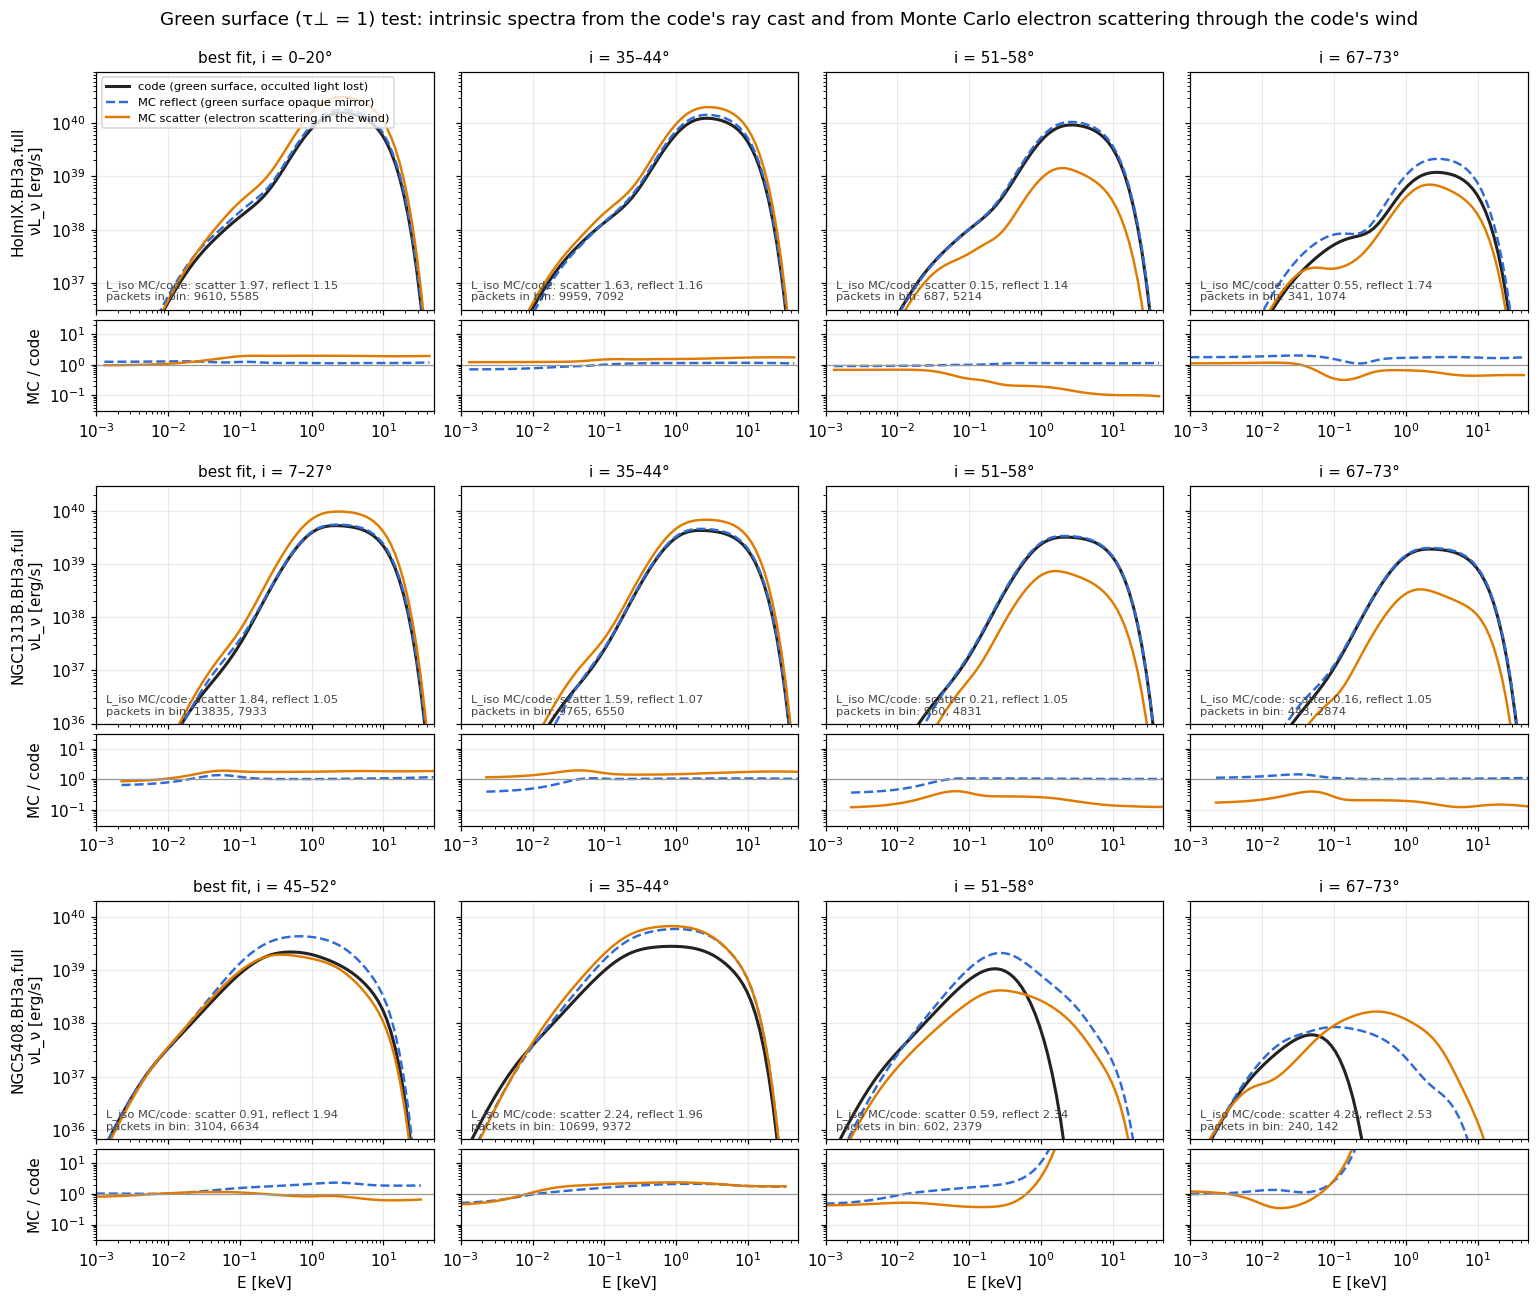
\includegraphics[width=\textwidth]{mc_green_surface_spectra.png}
\caption{Intrinsic spectra $\nu L_\nu$ (no absorption) of the best fits of \srcHoIX, \srcNGCthirteen and \srcNGCfiftyfour (rows; preset BH3a, full energy range) in bins $\mu \pm 0.05$ around the best-fit inclination, $40^\circ$, $55^\circ$ and $70^\circ$ (columns).
Black: the ray cast of the code (surface $\taup = 1$, occulted light lost).
Blue dashed: Monte Carlo with the surface $\taup = 1$ as an opaque diffuse mirror.
Orange: Monte Carlo with electron scattering in the wind of the model.
The lower panels show the ratio of the Monte Carlo to the ray cast.
Made with \code{docs/scripts/mc\_green\_surface.py} and \code{mc\_green\_surface\_spectra.py} (code commit fa567f9).}
\label{fig:mc_spectra}
% figure: ULXspectra docs/figures/mc_green_surface_spectra.png, commit fa567f9 (unchanged at 4da7c04)
\end{figure*}

\subsection{Collimation by the funnel: comparison with Ahlberg et al.}
\label{app:mc:funnel}

\citet{Ahlberg2026} computed the geometric beaming by a funnel in the shape of a conical frustum with infinitely optically thick, conservative walls and a point source at the centre of its base.
Their walls re-emit as Lambertian surfaces or reflect as an electron-scattering atmosphere; the two differ in the boost by at most 6 per cent.
% source: docs/green_surface_monte_carlo.md, "Funnel collimation from Ahlberg et al. (2026)", "Their model"
They define the boost of the apparent luminosity $B(i)$ by $L_{\rm app}(i) = B(i) \int F\,{\rm d}\Omega$.
Averaged over $i \le \alpha$, where $\alpha$ is the half-opening angle of the funnel, its geometric limit is (their Eq.~7)
\begin{equation}
B_{\rm max} = \frac{1}{1 - \cos\alpha} ,
\label{eq:mc_Bmax}
\end{equation}
% source: Ahlberg et al. 2026, Eq. 7, as quoted in docs/green_surface_monte_carlo.md
and the mean boost inside the funnel is approximated to about 10 per cent by (their Eq.~15)
\begin{equation}
\frac{\ln B}{\ln B_{\rm max}} \approx \exp\left(1.14\,\frac{\ln\sin\alpha}{\ln R}\right) ,
\label{eq:mc_AhlbergB}
\end{equation}
% source: Ahlberg et al. 2026, Eq. 15, as quoted in docs/green_surface_monte_carlo.md
where $R$ is the distance from the centre of the base to the edge of the funnel in units of the base radius.
% VERIFY: Eqs. (mc_Bmax), (mc_AhlbergB) against arXiv:2610.23089
In our wind, the innermost streamline is a straight cone at $\theta_{\rm c}$ from the axis starting at $\rin$, which is their geometry with $\alpha = \theta_{\rm c} = 45.6^\circ$.
% source: docs/green_surface_monte_carlo.md, "Comparison with our MC"

We first reproduced their setup with a Monte Carlo of our own (\code{docs/scripts/funnel\_beaming\_mc.py}): a conical frustum with Lambertian walls, an isotropic point source, and the plane $z = 0$ as a mirror for the lower half of the funnel, $4\times10^4$ packets per point.
% source: funnel_beaming_mc.py docstring and cone_mc(alpha, R, n=40000) for the validation; commit 4da7c04
The mean boost in the funnel agrees with their Eq.~\eqref{eq:mc_AhlbergB} within 1--13 per cent (Fig.~\ref{fig:funnel_validation}); Eq.~\eqref{eq:mc_AhlbergB} lies above our points at small $R$ and below them at large $R$, as \citet{Ahlberg2026} note.
Against their Fig.~4b, read by eye, we obtain $B/B_{\rm max} = 0.90$ at $R = 10^2$ and 0.96 at $R = 10^3$ for $\alpha = 45^\circ$ (theirs: 90 per cent at $R \approx 2\times10^2$, 95 per cent at $R \approx 1.5\times10^3$), 0.73 for $\alpha = 25^\circ$ and $R = 10^3$ (theirs about 72 per cent), and 0.31 for $\alpha = 10^\circ$ and $R = 10^3$ (theirs about 33 per cent).
For the narrow and long funnel $\alpha = 10^\circ$, $R = 10^5$, our 0.50 (Eq.~\ref{eq:mc_AhlbergB}: 0.51) is about 20 per cent above the 0.40--0.42 of their figure and text; we have no explanation, but the difference is irrelevant for $\alpha \approx 46^\circ$.
% source: docs/green_surface_monte_carlo.md, "Our opaque-cone MC vs Ahlberg et al."; commit 4da7c04

\begin{figure}
\centering
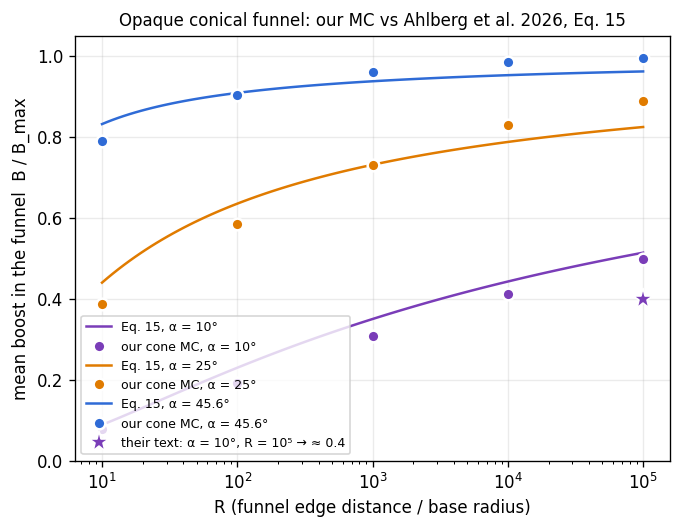
\includegraphics[width=\columnwidth]{funnel_beaming_validation.png}
\caption{Mean boost inside an opaque conical funnel, $B/B_{\rm max}$, against the distance $R$ of the funnel edge in units of the base radius, for $\alpha = 10^\circ$, $25^\circ$ and $45.6^\circ$.
Lines: Eq.~\eqref{eq:mc_AhlbergB} \citep[Eq.~15 of][]{Ahlberg2026}; dots: our Monte Carlo in their setup; star: the value quoted by \citet{Ahlberg2026} for $\alpha = 10^\circ$, $R = 10^5$.
Made with \code{docs/scripts/funnel\_beaming\_mc.py} (code commit 4da7c04).}
\label{fig:funnel_validation}
% figure: ULXspectra docs/figures/funnel_beaming_validation.png, commit 4da7c04
\end{figure}

The scattering case of Sect.~\ref{app:mc:method} agrees with the opaque cone in the mean (Table~\ref{tab:mc_funnel}).
For $\alpha = 45.6^\circ$ and $R = 10^2$--$10^4$, Eq.~\eqref{eq:mc_AhlbergB} gives $B = 3.02$--$3.17$ ($B_{\rm max} = 3.33$), and our wind gives 2.92--3.05, with 88--92 per cent of the light escaping inside the funnel.
The agreement is about 5 per cent, although the walls of our funnel are semi-transparent (2--32 scatterings in the median, Table~\ref{tab:mc_fits}) and our source is extended, the disc under the wind or the wind photosphere, rather than a point.
% source: docs/green_surface_monte_carlo.md, "Comparison with our MC" table and paragraph; commit 4da7c04

\begin{table}
\centering
\caption{Collimation by the funnel, $\alpha = \theta_{\rm c} = 45.6^\circ$: share of the light escaping at $i < \theta_{\rm c}$ and the mean boost $B$ there.}
\label{tab:mc_funnel}
\small
\begin{tabular}{@{}lcc@{}}
\toprule
& share at $i < \theta_{\rm c}$ & $B$ \\
\midrule
Eq.~\eqref{eq:mc_AhlbergB}, $R = 10^2$--$10^4$ & 1 & 3.02--3.17 \\
\srcHoIX, scattering & 0.91 & 3.04 \\
\srcNGCthirteen, scattering & 0.88 & 2.92 \\
\srcNGCfiftyfour, scattering & 0.92 & 3.05 \\
reflection (all three) & 0.54--0.79 & 1.8--2.6 \\
\bottomrule
\end{tabular}
% source: docs/green_surface_monte_carlo.md, "Comparison with our MC (scatter mode, 2026-10-31)"; commit 4da7c04
\end{table}

The angular distributions differ more than the means (Fig.~\ref{fig:funnel_wind}).
Inside the funnel, $B(i) = L_{\rm iso}(i)/L_{\rm total}$ of the wind is steeper than that of the opaque cone: 3.6--3.8 near the axis (cone 3.3--3.5) and 2.2--2.5 just inside the edge (cone 2.9).
Beyond $\theta_{\rm c}$ the wind leaks light with $B \approx 0.1$--$0.7$, and the opaque cone almost none.
% source: docs/green_surface_monte_carlo.md, "B(i) cone vs wind"; commit 4da7c04
The light emitted at different radii is collimated alike: inside the funnel its $B(i)$ is the same within about 10 per cent (Fig.~\ref{fig:funnel_radius}).
Only the outermost wind photosphere of \srcNGCfiftyfour ($x > 300$, 25 per cent of the luminosity) gives a flatter $B(i)$ and leaks more.
% source: docs/green_surface_monte_carlo.md, "B(i) by emission radius"; commit 4da7c04
For this reason the share of the luminosity above 1~keV in the Monte Carlo is constant within 1--2 per cent inside the funnel.
In the ray cast it is constant as well, because the directly seen surface is nearly flat and all rings scale as $\cos i$.
Beyond $\theta_{\rm c}$ the Monte Carlo spectrum is softer than inside, because the hot centre is hidden.
% source: docs/green_surface_monte_carlo.md, "Spectral shape against i"; commit 4da7c04

\begin{figure}
\centering
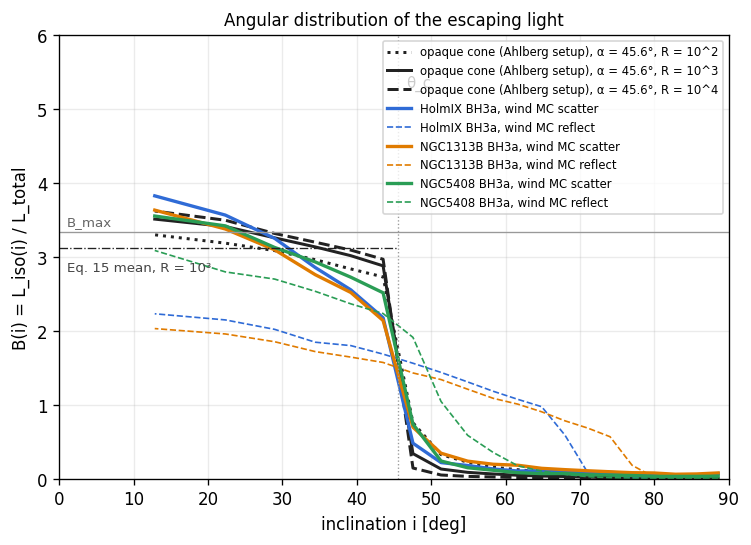
\includegraphics[width=\columnwidth]{funnel_beaming_vs_wind.png}
\caption{Angular distribution of the escaping light, $B(i) = L_{\rm iso}(i)/L_{\rm total}$, in 20 bins in $\mu$.
Black: opaque cone in the setup of \citet{Ahlberg2026}, $\alpha = 45.6^\circ$, $R = 10^2$, $10^3$, $10^4$.
Colours: Monte Carlo through the wind of the three best fits, scattering (solid) and reflection (dashed).
Made with \code{docs/scripts/funnel\_beaming\_mc.py} (code commit 4da7c04).}
\label{fig:funnel_wind}
% figure: ULXspectra docs/figures/funnel_beaming_vs_wind.png, commit 4da7c04
\end{figure}

\begin{figure*}
\centering
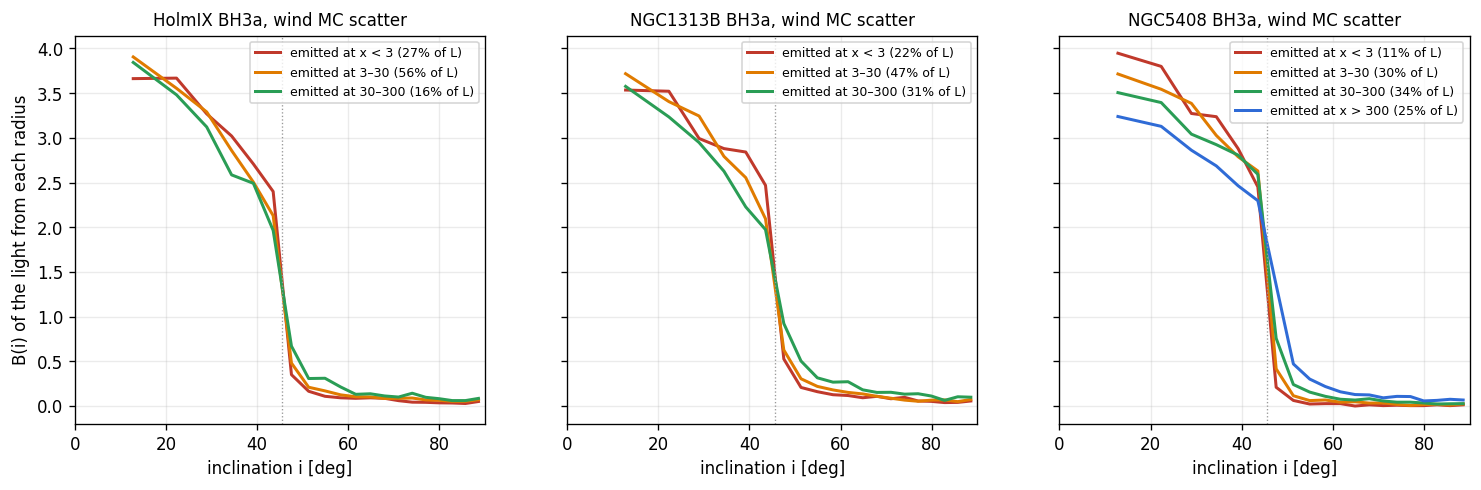
\includegraphics[width=\textwidth]{funnel_beaming_by_radius.png}
\caption{$B(i)$ of the light emitted at different radii $x = R/\rin$, Monte Carlo with scattering through the wind of the three best fits; the share of the luminosity emitted in each range is given in the legends.
The dotted line marks $\theta_{\rm c}$.
Made with \code{docs/scripts/funnel\_beaming\_mc.py} (code commit 4da7c04).}
\label{fig:funnel_radius}
% figure: ULXspectra docs/figures/funnel_beaming_by_radius.png, commit 4da7c04
\end{figure*}

\subsection{Limits of the test}
\label{app:mc:limits}

These results are preliminary.
The scattering is grey: isotropic Thomson scattering, without the Rayleigh phase function, without Doppler shifts or bulk Comptonization by the outflow, and without thermal Comptonization.
There is no absorption: a packet keeps the energy of the element that emitted it, and there is no thermalisation below the surface.
The disc plane has the albedo of unity.
The packets start on the surfaces of the model, so the test covers the transfer after emission, not where the light is emitted.
With $4\times10^4$ packets per run, a few hundred packets fall into each bin at $i \ge 70^\circ$.
% source: docs/green_surface_monte_carlo.md, "Limits of the Monte Carlo"
Only the BH fits were tested.
For a NS the Monte Carlo needs the disc surface ($\hd > 0$) and the magnetosphere as emitters and reflectors, the base of the funnel at the inner launch radius of the wind, and, for the central emitter up to about 30~keV, energy change in scattering.
% source: docs/green_surface_monte_carlo.md, "Limits" (BH fits only) and "NS fits"

% OUTLINE: what follows for the fits is the author's decision (docs/green_surface_monte_carlo.md,
%          "Possible next steps"; PLAN.md C18): inclination prior i < theta_c; energy conservation
%          in the ray cast; attenuation exp(-tau_los) along the line of sight; MC-calibrated
%          angular redistribution b(i; alpha, R) from the opaque cone + f_leak from the wind MC.
% AUTHOR: state here which of these (if any) the paper adopts, or move to the Discussion.


\bibliographystyle{plainnat}
\bibliography{refs}

\end{document}
